\documentclass[spanish]{beamer}
\usepackage[ansinew]{inputenc} % Acepta caracteres en castellano
\usepackage[spanish]{babel}    % silabea palabras castellanas
\usepackage{amsmath}
\usepackage{amsfonts}
\usepackage{amssymb}
\usepackage{dsfont}
\usepackage{graphicx}
\usepackage{geometry}
\usetheme{Madrid}
\usecolortheme{beaver}
\usepackage{textpos}
% Logo  en el comienzo 
\addtobeamertemplate{frametitle}{}{%
\begin{textblock*}{100mm}(.85\textwidth,-1cm)
{\includegraphics[height=0.4in, keepaspectratio=true]{/Users/luisnunez/Dropbox/MisDocumentos/UIS/UISImagenInstitucional/UISLOGO.png}}
\end{textblock*}}

\begin{document}

\title{\textbf{Principios Variacionales} }
\author[L.A. N��ez]{\textbf{Luis A. N��ez}}  
\institute[UIS]{\textit{Escuela de F�sica, Facultad de Ciencias, } \\
\textit{Universidad Industrial de Santander, Santander, Colombia } \\
{\includegraphics[height=0.4in, keepaspectratio=true]{/Users/luisnunez/Dropbox/MisDocumentos/UIS/UISImagenInstitucional/UISLOGO.png}}
}
\date{\today}
\maketitle


\begin{frame}
\frametitle{Agenda}
  \tableofcontents
\end{frame}


%%%%% Diapo 1
  \section{Extremos de un funcional}
\frame{
  \frametitle{Extremos de un funcional}
   \begin{itemize}  
  	\item<1-> En los problemas de extremos del c�lculo diferencial se busca el valor de una variable $x$ para el cual una funci�n $y = g(x)$ es m�xima o m�nima. 
  	\item<2-> En los problemas de extremos en el c�lculo variacional se busca una funci�n $f(x)$ con cual un funcional, $I=\mathcal{F}[f(x)]$, sea extremo (m�ximo o m�nimo). 
	\item<3-> Entonces anularemos las variaciones del funcional, $\delta I = \delta \mathcal{F}[f(x)] = 0$, para determinar la $f(x)$ que lo hace extremo.
			\begin{figure}[t]
			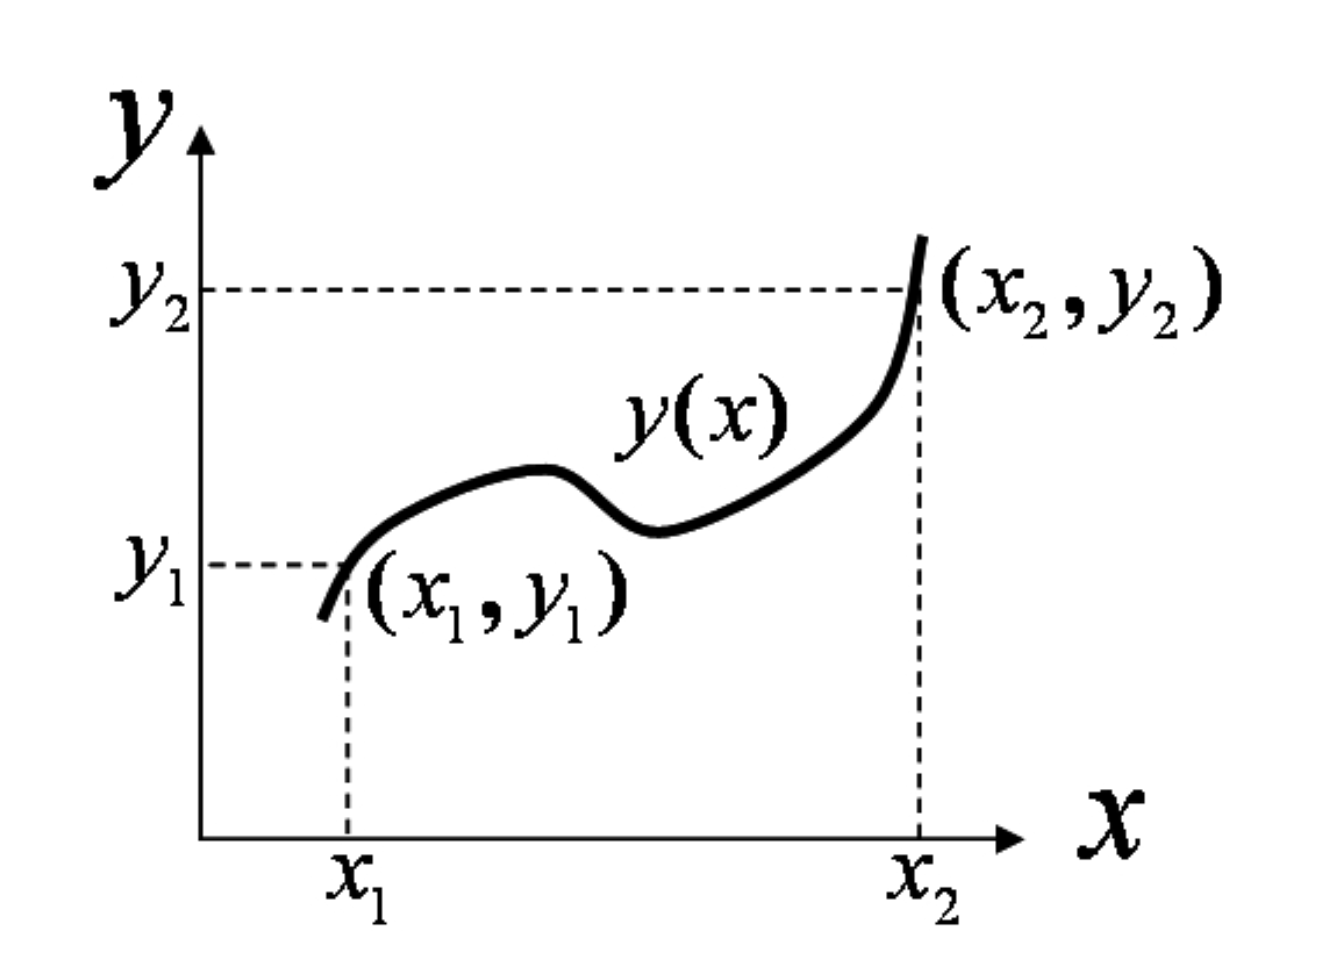
\includegraphics[width=1.4in]{Figuras/Trayectoria.png} \hspace{1cm} 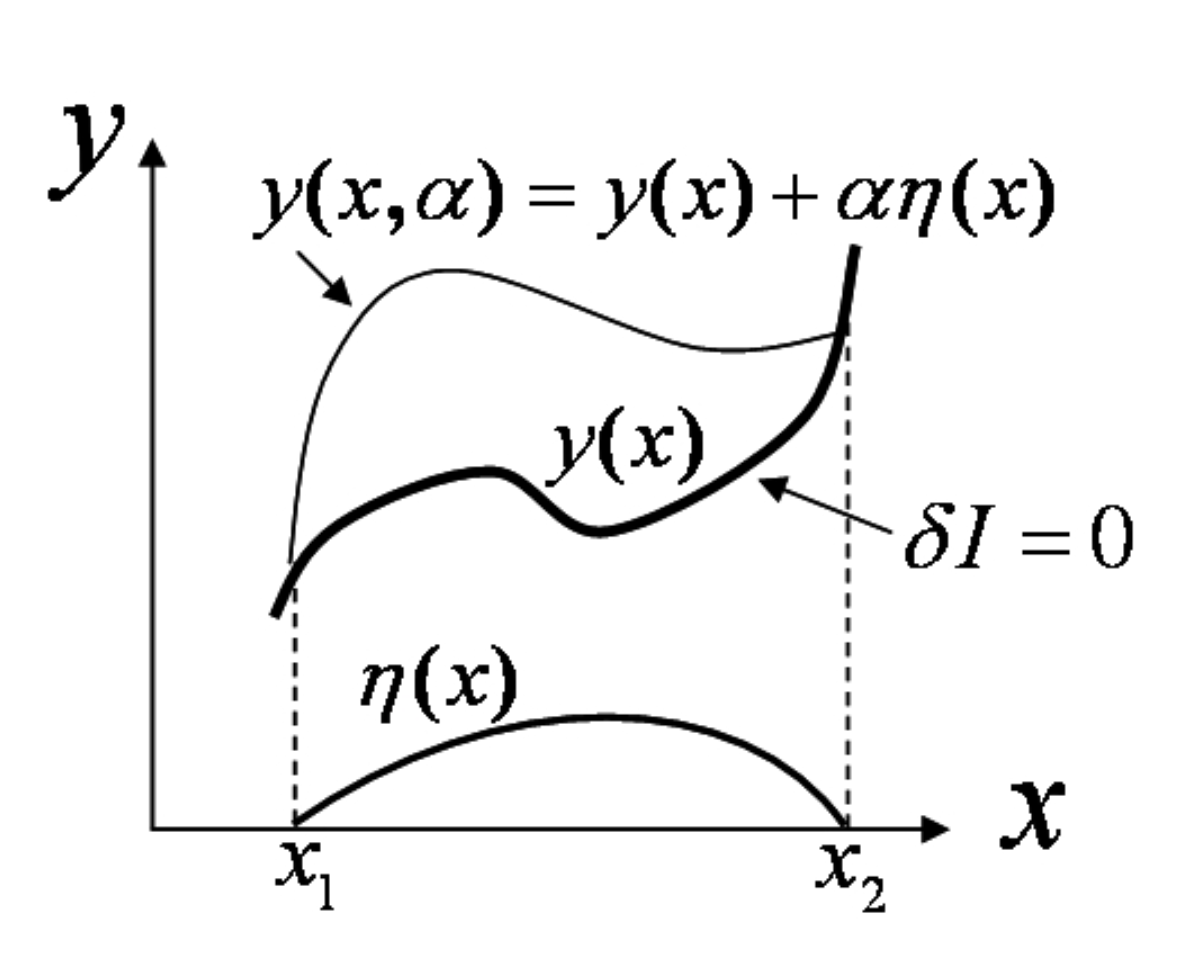
\includegraphics[width=1.4in]{Figuras/TrayectoriaPerturbada.png} 
   		         \end{figure}
    \end{itemize}
}
%%%%% Diapo 2
\section{Trayectorias cercanas a la extrema}
\frame{
  \frametitle{Trayectorias cercanas a la extrema}
  \begin{itemize}  
  	\item<1->  Sea $y(x)$ la funci�n que hace extremo el funcional $I = \mathcal{F}[f(x)] = \int_{x_1}^{x_2} {\rm d}x \; f(y(x), y^{\prime}(x), x)$. 
	\item<2->  Consideremos todas las funciones cercanas a $y(x)$ de la forma $y(x,\alpha) = y(x) + \alpha \eta(x)$, con lo cual $y(x, 0) = y(x)$
	\item<3->  La funci�n $\eta(x)$ es diferenciable y $\eta(x_1) = \eta(x_2) = 0$, con lo cual $y(x_1, 0) = y(x_1) \equiv y_1$ y consecuentemente $y(x_2, 0) = y(x_2) \equiv y_2$
	\item<4->  Entonces hemos transformado el funcional en una funci�n $I(\alpha) = \mathcal{F}[f(x, \alpha)] = \int_{x_1}^{x_2} {\rm d}x \; f(y(x, \alpha), y^{\prime}(x, \alpha), x)$
	\item<5-> Sabemos como buscar los extremos de una funci�n $\left.\frac{{\rm d} I(\alpha)}{{\rm d} \alpha}\right|_{\alpha=0} = 0$
	\item<6-> Al evaluar $\alpha = 0$ garantizamos que obtenemos la $y(x)$ que hace extremo el funcional $I$.  
  \end{itemize}
}

%%%%% Diapo 3
\section{Variaciones de un funcional}
\frame{
  \frametitle{Variaciones de un funcional}
  \begin{itemize}  
  	\item<1-> La derivada $\frac{{\rm d} I(\alpha)}{{\rm d} \alpha} = \int_{x_1}^{x_2} \frac{{\rm d} f\left(y(x, \alpha), y^{\prime}(x, \alpha), x\right)}{{\rm d} \alpha} {\rm d} x$
	\item<2-> Equivalentemente $\frac{{\rm d} I(\alpha)}{{\rm d} \alpha} = \int_{x_1}^{x_2}\left[\frac{\partial f}{\partial y} \frac{\partial y(x, \alpha)}{\partial \alpha}+\frac{\partial f}{\partial y^{\prime}} \frac{\partial y^{\prime} (x, \alpha)}{\partial \alpha} \right] {\rm d} x $
	\item<3-> Donde $\frac{\partial y(x, \alpha)}{\partial \alpha}  =\eta(x)$ y adem�s $\frac{\partial y^{\prime}(x, \alpha)}{\partial \alpha}  =\frac{\partial}{\partial \alpha}\left(\frac{{\rm d} y}{{\rm d} x}\right)=\frac{{\rm d}}{{\rm d} x}\left(\frac{\partial y}{\partial \alpha}\right)=\frac{{\rm d} \eta}{{\rm d} x}$
	\item<4-> Con lo cual $\frac{{\rm d} I}{{\rm d} \alpha}=\int_{x_1}^{x_2}\left[\frac{\partial f}{\partial y} \eta(x)+\frac{\partial f}{\partial y^{\prime}} \frac{{\rm d} \eta}{{\rm d} x}\right] {\rm d} x .$
	\item<5-> El segundo t�rmino se integra por partes, $\int u v^{\prime} d x=u v-\int u^{\prime} v d x$,
	\item<5-> Esto es: $\int_{x_1}^{x_2} \frac{\partial f}{\partial y^{\prime}} \frac{{\rm d} \eta}{{\rm d} x} {\rm d} x= 
	\underbrace{\left.\frac{\partial f}{\partial y^{\prime}} \eta(x)\right|_{x_1} ^{x_2}}_{=0} -\int_{x_1}^{x_2} \frac{{\rm d}}{{\rm d} x}\left(\frac{\partial f}{\partial y^{\prime}}\right) \eta(x) {\rm d} x,$
	\item<6-> Finalmente $\frac{{\rm d} I}{{\rm d} \alpha}=\int_{x_1}^{x_2}\left[\frac{\partial f}{\partial y}-\frac{{\rm d}}{{\rm d} x}\left(\frac{\partial f}{\partial y^{\prime}}\right)\right] \eta(x) {\rm d} x .$
   \end{itemize}
}
%%%%% Diapo 4
\section{La ecuaci�n de Euler}
\frame{
  \frametitle{La Ecuaci�n de Euler}
  \begin{itemize}  
  	\item<1-> Evaluando en $\alpha=0$, tenemos $\left.\frac{{\rm d} I}{{\rm d} \alpha}\right|_{\alpha=0}=\int_{x_1}^{x_2}\left[\frac{\partial f}{\partial y}-\frac{{\rm d}}{{\rm d} x}\left(\frac{\partial f}{\partial y^{\prime}}\right)\right]_{\alpha=0} \eta(x) {\rm d} x=0 .$
	\item<2-> La condici�n $\left.\frac{d I}{d \alpha}\right|_{\alpha=0}=0$ implica que el integrando se anula.
	\item<3-> Con lo cual $\frac{d}{d x}\left(\frac{\partial f}{\partial y^{\prime}}\right)-\frac{\partial f}{\partial y}=0$
	\item<4-> La ecuaci�n de Euler expresa la condici�n que debe satisfacer la funci�n $y(x)$ para que el funcionl $I$ sea extremo. 
	\item<5-> Es una ecuaci�n diferencial de segundo orden para $y(x)$ para las condiciones dadas.
   \end{itemize}
}


  
\end{document}

%%%%% Diapo 2
\section{Secci�n}
\frame{
  \frametitle{T�tulo transparencia}
  \begin{itemize}  
  	\item<1-> 
   \end{itemize}
}
%%%%% Diapo 2
\section{Secci�n}
\frame{
  \frametitle{T�tulo transparencia}
  \begin{itemize}  
  	\item<1-> 
   \end{itemize}
}
%%%%% Diapo 2
\section{Secci�n}
\frame{
  \frametitle{T�tulo transparencia}
  \begin{itemize}  
  	\item<1-> 
   \end{itemize}
}

%%%%% Diapo Fin
\section{Recapitulando}
\frame{
  \frametitle{Recapitulando}
En presentaci�n consideramos
  \begin{enumerate}
  \item<1->
    \end{enumerate}
}



